\part{Vertices and Elements}
\frame{\partpage}

\begin{frame}[fragile]{Vertex Data}
	\begin{itemize}
		\pause\item Vertices  always have a \textbf{position}, but may also have other data associated, e.g. colour.
		\pause\item One way we could store this data is to use a separate Vertex Buffer for each \textbf{attribute}:
	\end{itemize}
	\pause\begin{lstlisting}
	struct Vertex { float x,y,z; };
	Vertex v[]={{-0.5f,-0.5f,0.0f},
			{0.5f,-0.5f,0.0f},
			{0.0f,0.5f,0.0f}};

	struct Colour { float r,g,b,a; };
	Colour c[]={{1.0f,0.0f,0.0f,1.0f},
			{0.0f,1.0f,0.0f,1.0f},
			{0.0f,0.0f,1.0f,1.0f}};
	\end{lstlisting}
\end{frame}

\begin{frame}[fragile]{Using Separate Vertex Buffers}
	\begin{lstlisting}
GLuint vertexbuffers[2];
glGenBuffers(2, vertexbuffers);

// Set up vertex position buffer
glBindBuffer(GL_ARRAY_BUFFER, vertexbuffers[0]);
glBufferData(GL_ARRAY_BUFFER, sizeof(v), v, GL_STATIC_DRAW);
glEnableVertexAttribArray(0);
glVertexAttribPointer(0, 3, GL_FLOAT, GL_FALSE,
		3 * sizeof(GL_FLOAT), (void*)0);

// Set up vertex colour buffer
glBindBuffer(GL_ARRAY_BUFFER, vertexbuffers[1]);
glBufferData(GL_ARRAY_BUFFER, sizeof(c), c, GL_STATIC_DRAW);
glEnableVertexAttribArray(1);
glVertexAttribPointer(1, 4, GL_FLOAT, GL_FALSE,
		4 * sizeof(GL_FLOAT), (void*)0);
	\end{lstlisting}
\end{frame}
	
\begin{frame}[fragile]{Interleaved Vertices}
	\begin{itemize}
		\pause\item Alternatively, we can create a \textbf{C structure} which represents a Vertex, which has member variables which represent positions, colours, normals etc.
		\pause\item This is known as \textbf{Interleaved Vertices} and in \textbf{MOST} cases is more efficient.
	\end{itemize}
	\pause\begin{lstlisting}
	struct Vertex
	{
		float x,y,z;
		float r,g,b,a;
	};
	
	Vertex v[]={{-0.5f,-0.5f,0.0f, 1.0f,0.0f,0.0f,1.0f},
				{0.5f,-0.5f,0.0f,  0.0f,1.0f,0.0f,1.0f},
				{0.0f,0.5f,0.0f,   0.0f,0.0f,1.0f,1.0f}};
	\end{lstlisting}
\end{frame}

\begin{frame}[fragile]{Using a Single Buffer}
	\begin{itemize}
		\pause\item We need to update the Vertex Attribute Array to interpret the data correctly:
		\begin{itemize}
			\pause\item Increase the \textbf{stride} for all attributes
			\pause\item Include the \textbf{offset} for everything but the position
		\end{itemize}
	\end{itemize}
	\pause\begin{lstlisting}
GLuint vertexbuffer;
glGenBuffers(1, &vertexbuffer);
glBindBuffer(GL_ARRAY_BUFFER, vertexbuffer);
glBufferData(GL_ARRAY_BUFFER, sizeof(v), v, GL_STATIC_DRAW);

glEnableVertexAttribArray(0);	// Position attribute
glVertexAttribPointer(0, 3, GL_FLOAT, GL_FALSE,
		sizeof(Vertex), (void*)0);

glEnableVertexAttribArray(1);	// Colour attribute
glVertexAttribPointer(1, 4, GL_FLOAT, GL_FALSE,
		sizeof(Vertex), (void*)(3 * sizeof(GL_FLOAT)));
	\end{lstlisting}
\end{frame}

\begin{frame}{Vertices in Memory}
	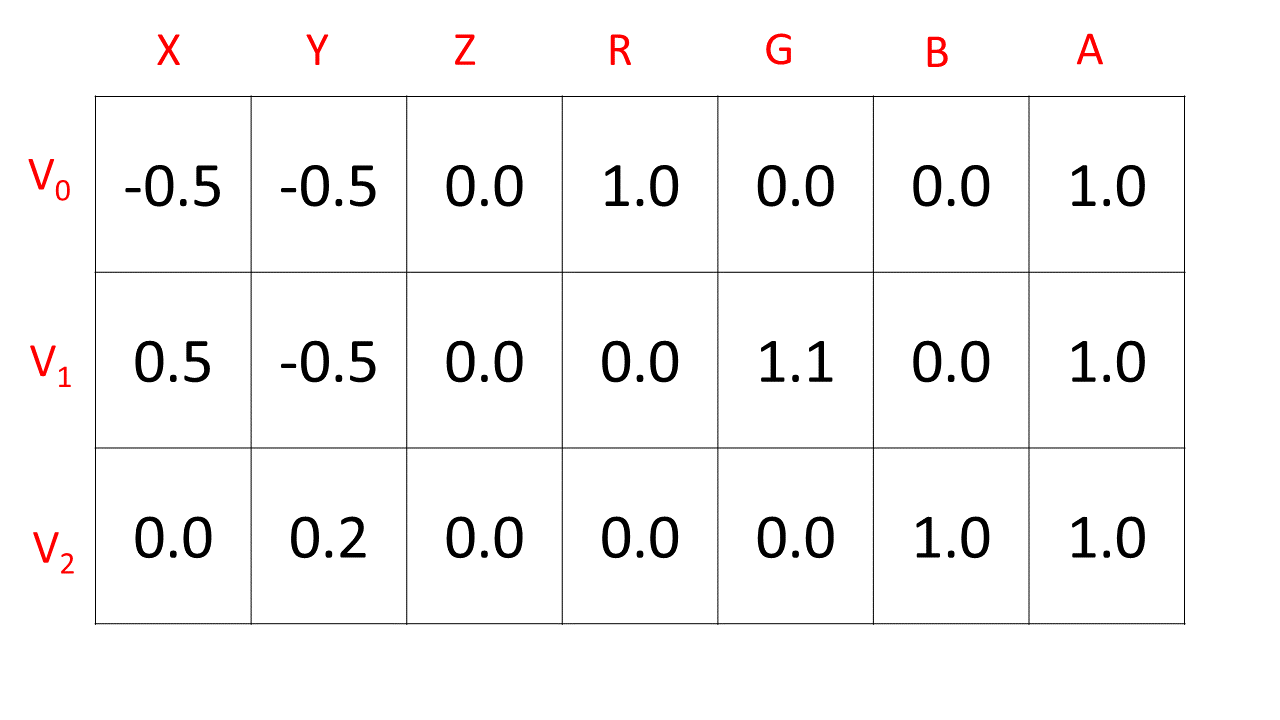
\includegraphics[width=1\textwidth]{MemoryLayoutValues}	
\end{frame}

\begin{frame}{Vertices in Memory: Stride}
	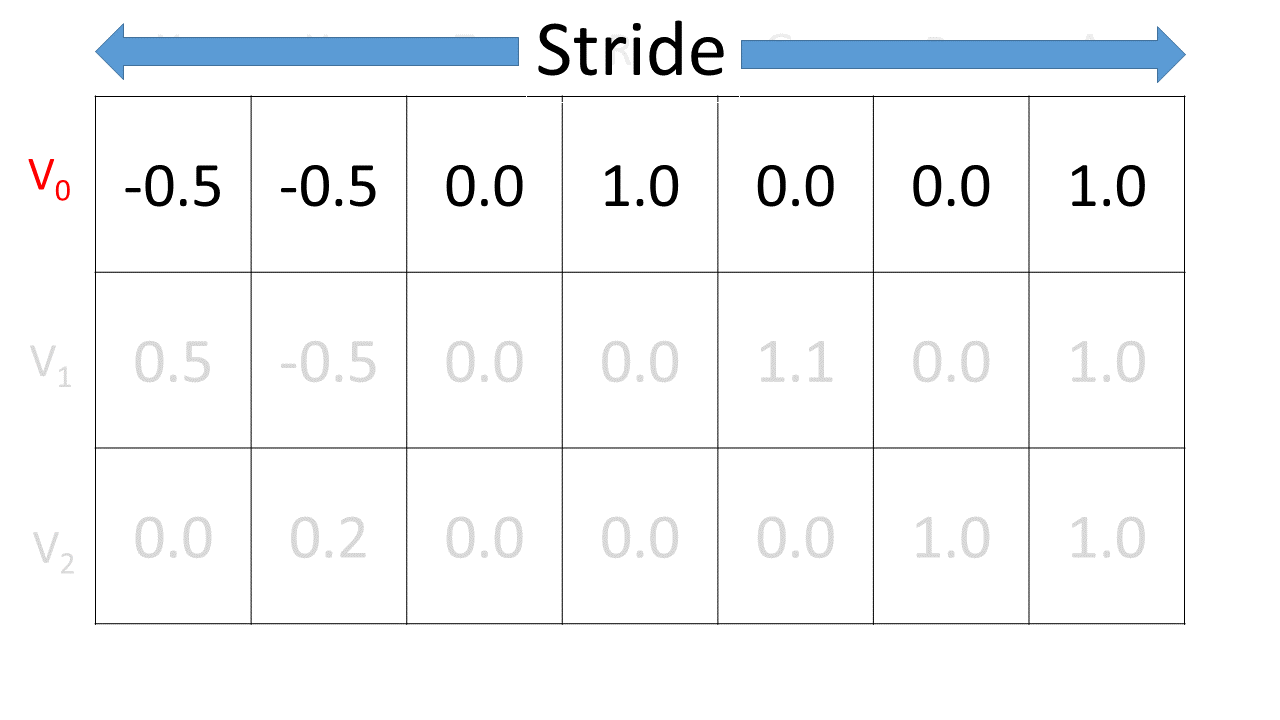
\includegraphics[width=1\textwidth]{MemoryLayoutStride}	
\end{frame}

\begin{frame}{Vertices in Memory: Offset}
	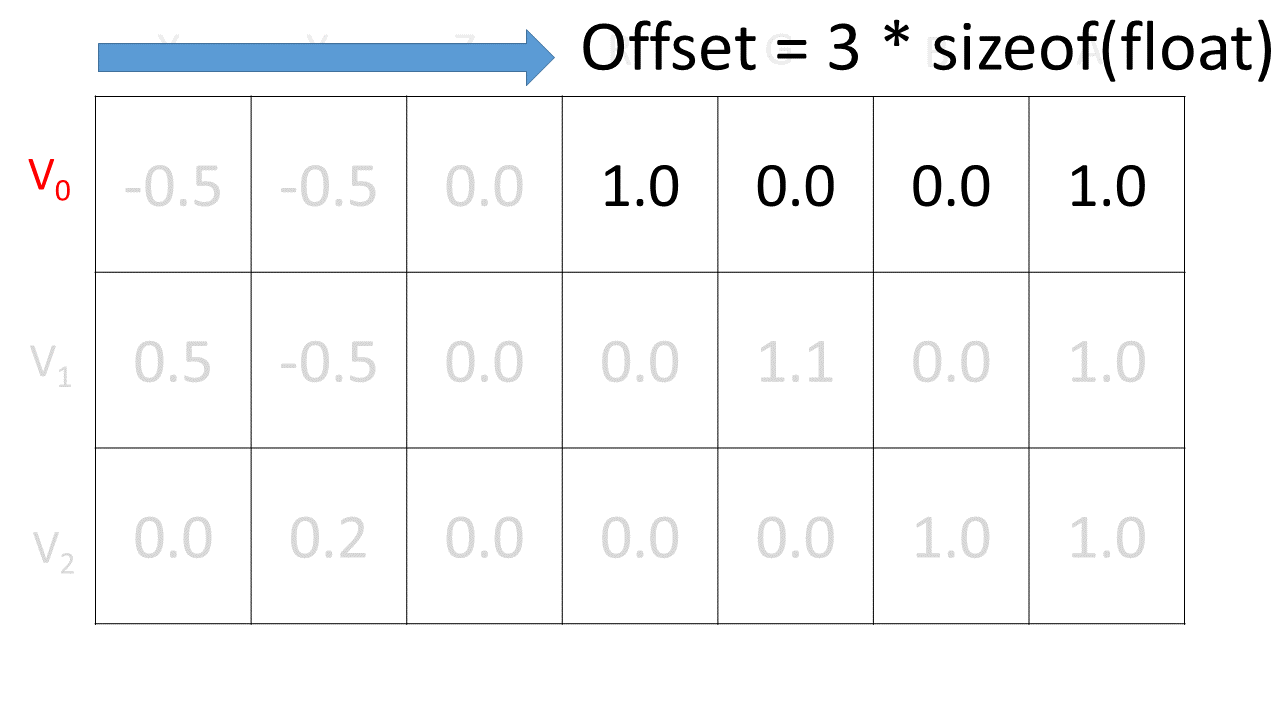
\includegraphics[width=1\textwidth]{MemoryLayoutOffset}	
\end{frame}

\begin{frame}{Multiple Triangles}
	\begin{itemize}
		\pause\item For the triangle, we listed each vertex's data in the buffer.
		\pause\item What if we have shapes made of multiple triangles (known as \textbf{meshes})?
	\end{itemize}
	\begin{columns}
		\begin{column}{0.5\textwidth}
			\begin{center}
				\pause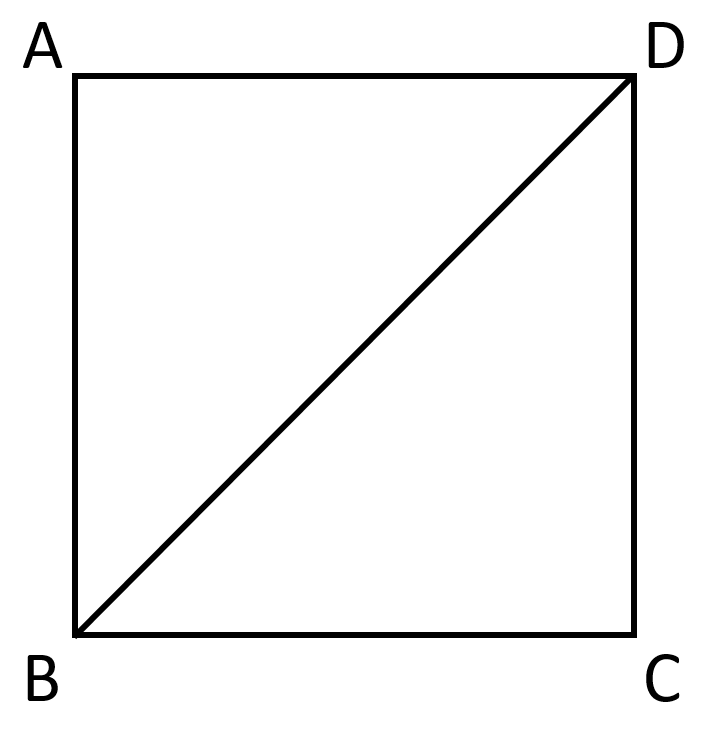
\includegraphics[height=0.3\textheight]{square_vertices}\\
				Square: 4 vertices\\
				2 triangles: 6 vertices
			\end{center}
		\end{column}
		\begin{column}{0.45\textwidth}
			\begin{center}
				\pause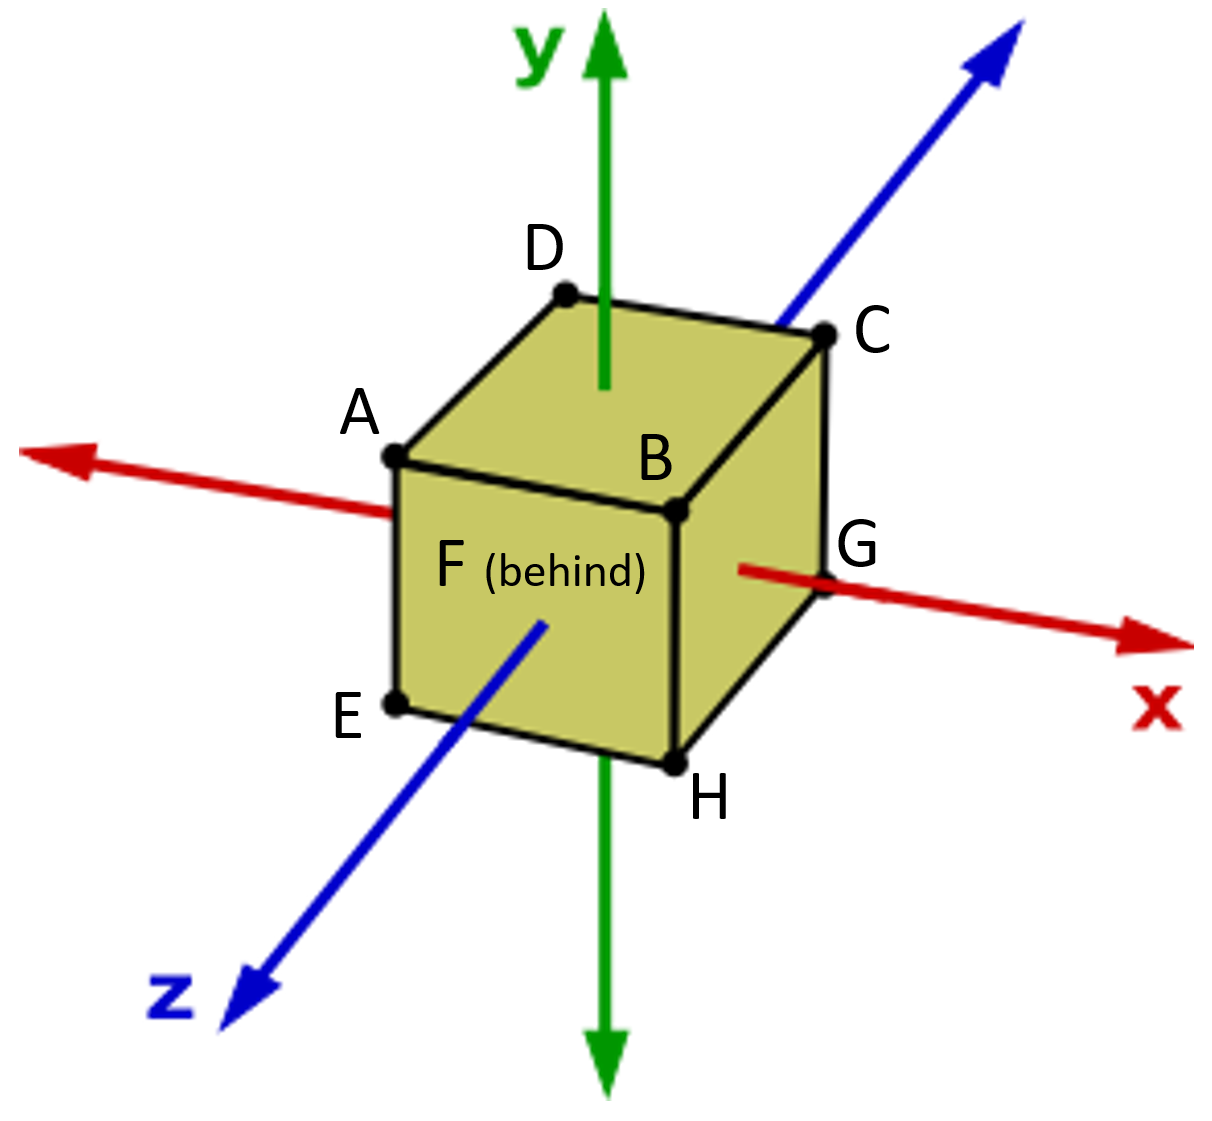
\includegraphics[height=0.3\textheight]{cube_vertices}\\
				Cube: 8 vertices\\
				12 triangles: 36 vertices\\
				(6 square faces)
			\end{center}
		\end{column}
	\end{columns}
\end{frame}

\begin{frame}{Element Buffer}
	\begin{itemize}
		\pause\item We can use an \textbf{Element Buffer} to optimise our drawing and avoid storing duplicate vertices.
		\pause\item An Element Buffer holds an integer which is an \textbf{offset} (or index) into a Vertex Buffer.
	\end{itemize}
	\begin{center}
		\pause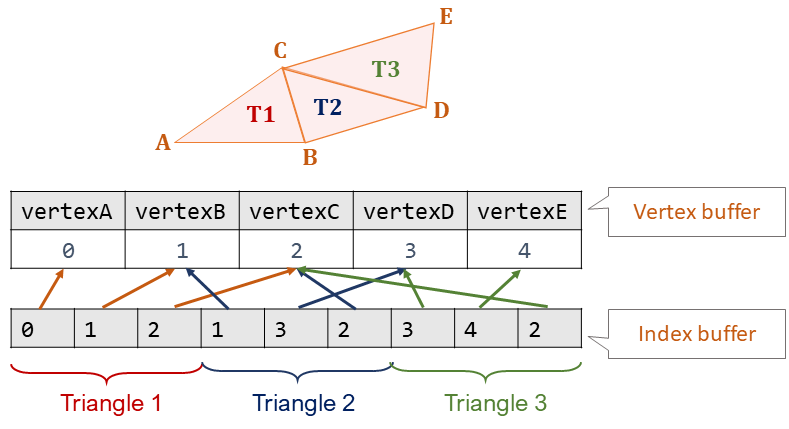
\includegraphics[height=0.5\textheight]{element_buffer}
	\end{center}	
\end{frame}

\begin{frame}{Vertex Order}
	\begin{itemize}
		\pause\item It is sometimes important to know which side of a triangle is the ``front'' and which is the ``back''
		\pause\item OpenGL determines this by \textbf{winding order}
	\end{itemize}
	\begin{columns}
		\pause
		\begin{column}{0.48\textwidth}
			\begin{center}
				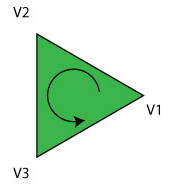
\includegraphics[width=0.5\textwidth]{winding_ccw}\\
				If the vertices go \textbf{anticlockwise}, you are looking at the \textbf{front}
			\end{center}
		\end{column}
		\pause
		\begin{column}{0.48\textwidth}
			\begin{center}
				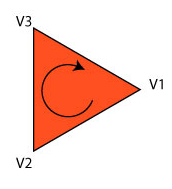
\includegraphics[width=0.5\textwidth]{winding_cw}\\				
				If the vertices go \textbf{clockwise}, you are looking at the \textbf{back}
			\end{center}
		\end{column}
	\end{columns}
\end{frame}

\begin{frame}[fragile]{Backface culling}
	\pause
	\begin{lstlisting}
glEnable(GL_CULL_FACE);
	\end{lstlisting}
	\begin{itemize}
		\pause\item This will cause only the front faces of triangles to be drawn
		\pause\item Triangles whose front face is not visible will be \textbf{culled}
		\pause\item Culled faces are not passed through the rasteriser or fragment shader
		\pause\item Saves time, and should make no difference to appearance ---
			as long as all meshes are closed and have correct winding
	\end{itemize}
\end{frame}

\begin{frame}[fragile]{When backface culling goes bad?}
	\begin{center}
		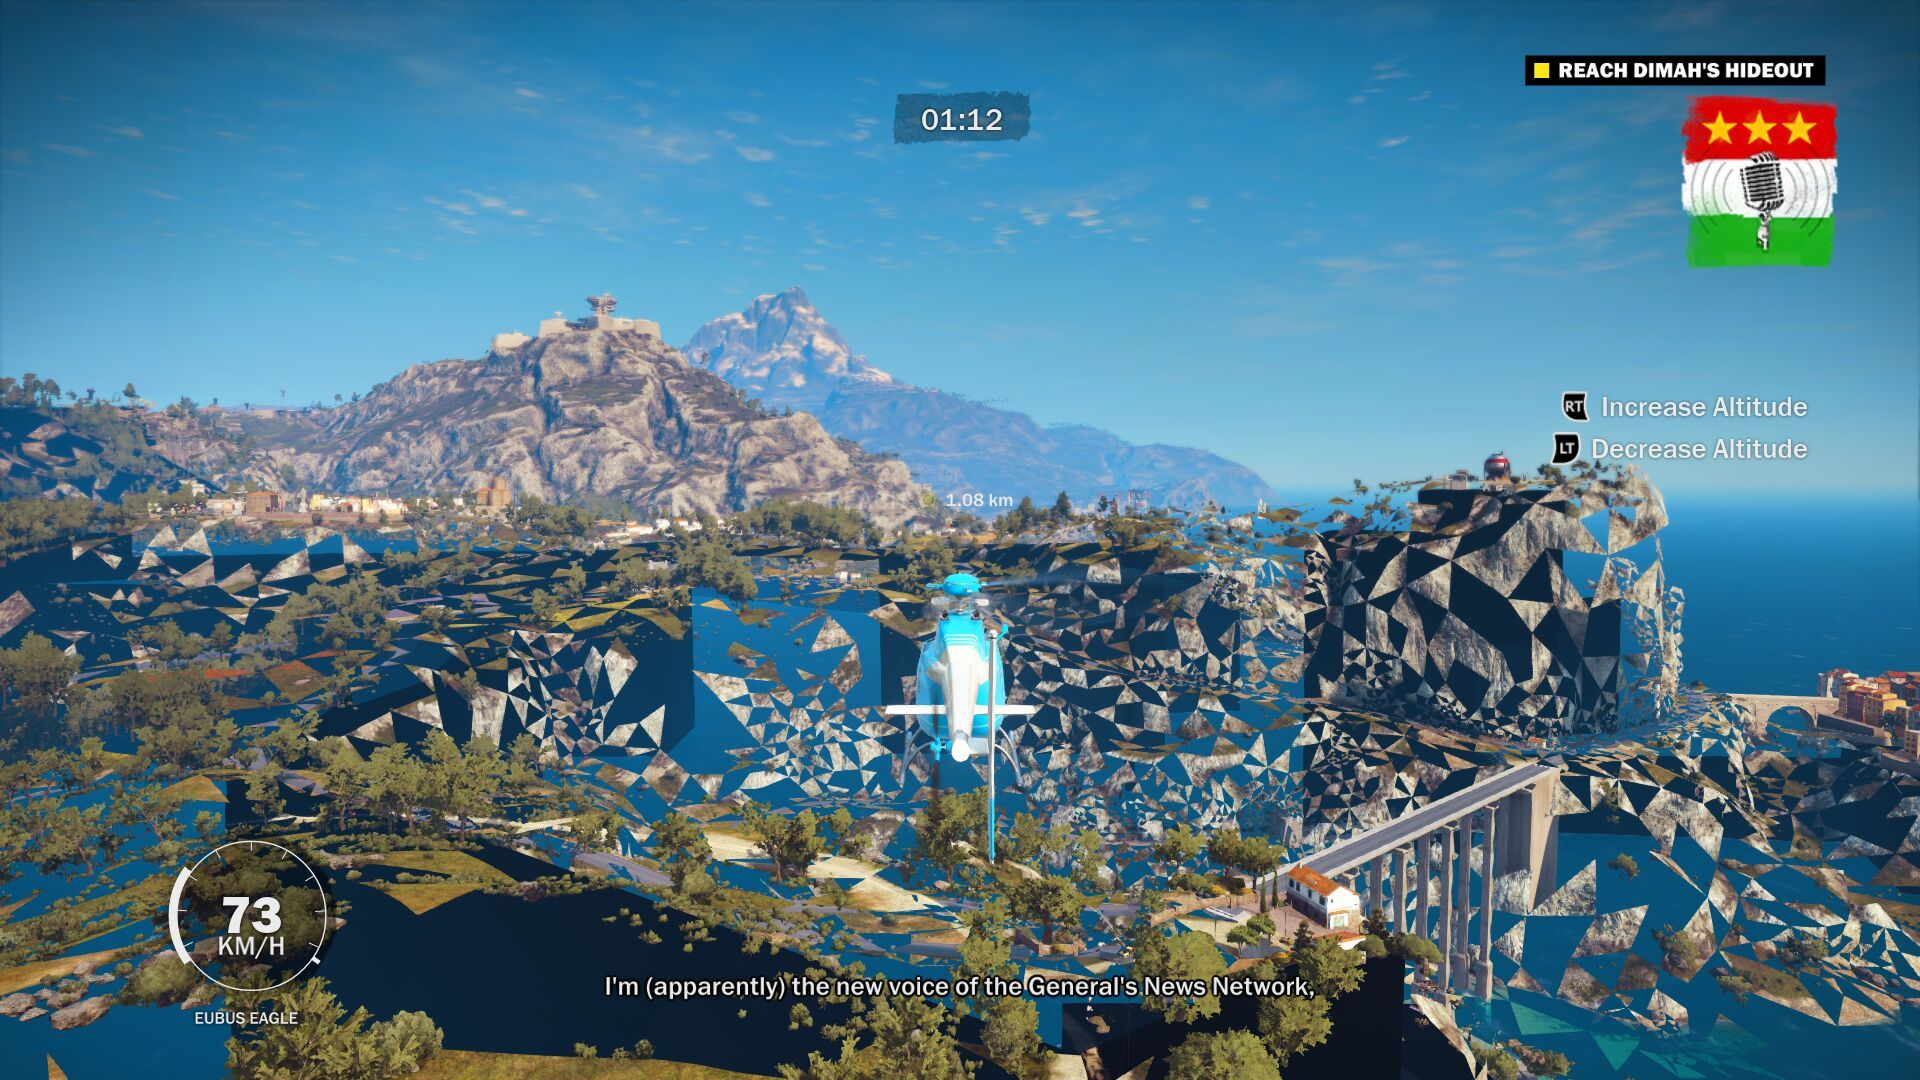
\includegraphics[width=\textwidth]{missing_triangles}
	\end{center}
\end{frame}



